\documentclass{utmthesis}
\usepackage{graphicx}
\usepackage{url} 
\usepackage[pages=some]{background}

\begin{document}

% Required information
\title{The Thesis Title}
\titletwo{Second Line (Optional)}
\titlethree{Third Line (Optional)}
\author{The Author}
\degree{Bachelor of Science}
\specialization{Physics}
\intakeyear{2011}
\faculty{Faculty of Science}
\titledate{July 2016}
\award{1}
% Options for Award 
% 1. Bachelor Degree Project Report
% 2. Master's Project Report (By course work)
% 3. Master's Dissertation (By course work and research)
% 4. Master's Thesis (By research)
% 5. Doctor of Philosophy Thesis
% 6. Other PhD Thesis
% 7. Generic PhD Thesis
% 8. Thesis Proposal
\superone{M.Y. Supervisor}
\supertwo{M.Y. Other Supervisor}
%\superthree{Third SV}
%\superfour{Fourth SV}
%\superfive{Fifth SV}

% Option for two-page printing
\newgeometry{top=2.5cm,left=4cm,right=2.5cm,bottom=2.5cm,twoside}

% Option to add watermark page
% Comment for final version	
\backgroundsetup{scale=1,angle=0,opacity=.1,hshift=0.25in,vshift=-0.5in,contents={
\includegraphics[width=5cm]{figs/utm02.jpg}}}
\watermarkpage

% Mandatory pages
\coverpage
\superpage
\certification
\frontmatter
\maketitle
\declaration


\begin{dedication}
Dedication\
\end{dedication}


\begin{acknowledgement}
Acknowledgement
\end{acknowledgement}


\begin{abstract}
This is the English abstract
\end{abstract}


\begin{abstrak}
Ini adalah abstrak Bahasa Melayu
\end{abstrak}


\tableofcontents
\listoftables
\listoffigures


%List of abbreviation 
\listofabbre
\addabbre{ANN}{Artificial Neural Network}
\addabbre{PC}{Personal Computer}
\addabbre{SVM}{Support Vector Machine}
\addabbre{XML}{Extensible Markup Language}


%List of symbols 
\listofsymbols
\addsymbol{$\gamma$}{Whatever}
\addsymbol{$\sigma$}{Whatever}
\addsymbol{$\varepsilon$}{Whatever}


%Uncomment if have appendices
\listofappendices

\onehalfspacing
\mainmatter


\chapter{Introduction}
\section{Problem Background}
Introduction to the thesis \cite{b2} to the thesis \cite{okamoto2004improved}. This section attempts to give a brief introduction to quantum computing. Before entering the microscopic world of quantum computing, we revisit the present digital system commonly used by the masses.  The current digital system is based on binary digits, commonly known as bits.  Each bit is represented with a binary value called ``logic 0'' or ``logic 1'' and the number of distinct states is $2^n$, where $n$ is the number of bits.  Physically, these logic values are typically represented by two different voltage levels. In this thesis, such computers are referred to as a \emph{classical computer}.
\section{State-of-the-Arts}
\section{Problem Statement}
\section{Objective and Scope}
\section{Organization}

% You can call another LaTeX document 
\chapter{Literature Review}
\label{chap:lit.review}

\section{State-of-the-Arts}

\section{Limitations}
\begin{enumerate}
\item Mentor~Graphics 2
\begin{enumerate}
\item item 3
\end{enumerate}
\item item 4
\end{enumerate}

\section{Research Gaps}
The processing at layer-5%
\footnote{In this thesis, OSI model is used.} is done ...



\chapter{Research Methodology}
\section{Top-level View}
\section{Research Activities}
\section{Controllables vs. Obseravables}
\section{Techniques}
\section{Tools and Platforms}
\section{Chapter Summary}


\chapter{Proposed Work}
\section{The Big Picture}
\section{Analytical Proofs}


\section{Results and Discussion}

\begin{figure}[p]
	\centering
	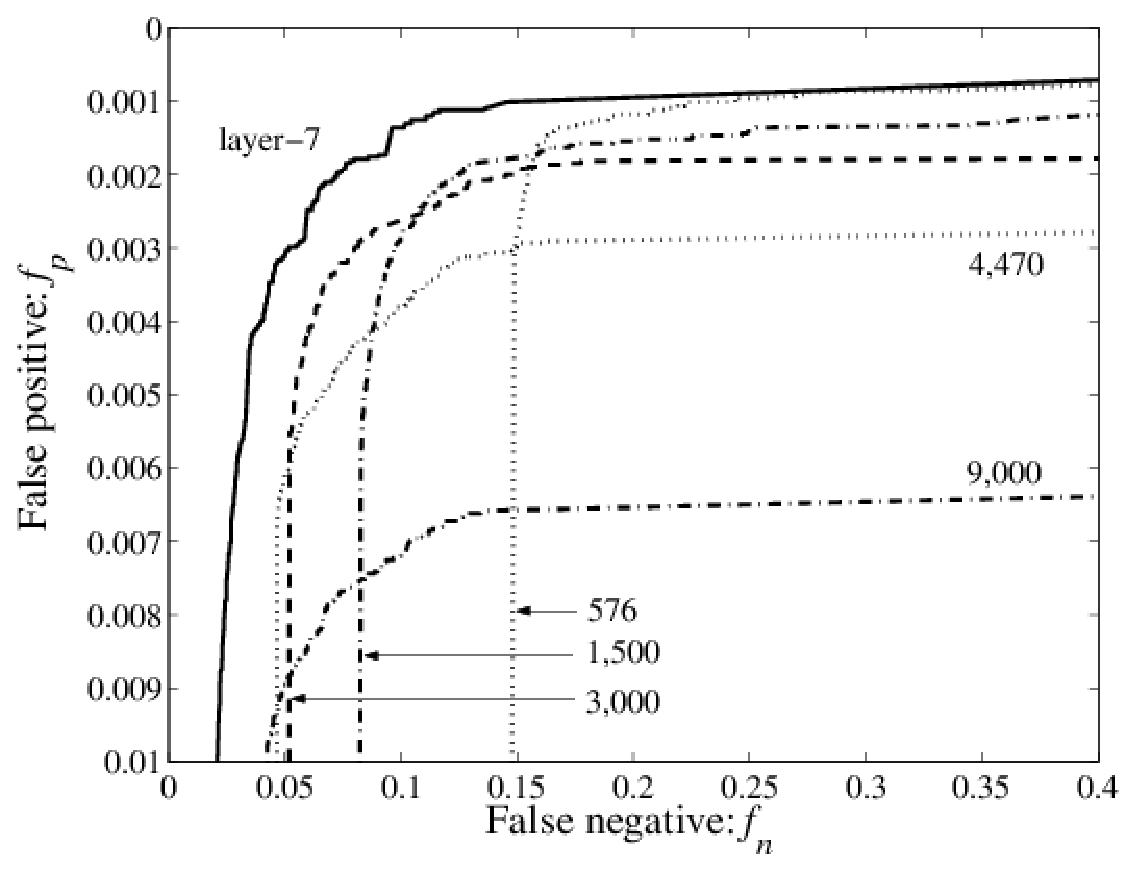
\includegraphics[width=\linewidth]{./figs/roc_TREC}
	\caption[Short version of the caption.]{Example of a figure. This is a long, very long, long long, long caption.  You can give a shorter caption for the ``list of figures" using the square braket symbol.}
\end{figure}


\begin{table}[p]
\centering
\caption[Short version of the caption.]{Example of a table. This is a long, very long, long long, long caption.  You can give a shorter caption for the ``list of table" using the square braket symbol.}
\vspace{\baselineskip}
\begin{tabular}{l c c}
  \hline
  \hline
  Temperature & Resonant Frequency & Q factor\\
  \hline
  13 mK $\pm$ 1 mK & 16.93 & 811 \\
  40 mK $\pm$ 1 mK & 16.93 & 817 \\
  100 mK $\pm$ 1 mK & 16.93 & 815 \\
  300 mK $\pm$ 1 mK & 16.93 & 806\\
  500 mK $\pm$ 1 mK & 16.93 & 811\\
  800 mK $\pm$ 5 mK & 16.93 & 814\\
  1000 mK $\pm$ 5 mK & 16.93 & 806 \\
  \hline
  \hline
\end{tabular}
\end{table}

\section{Chapter Summary}


\chapter{Conclusion}
\section{Research Outcomes}
\section{Contributions to Knowledge}
\section{Future Works}


\bibliographystyle{utmthesis-numbering}
\bibliography{reference}


\appendix
\chapter{Do not use long titles.}

\chapter{Pseudo-codes}

\chapter{Time-series Results}

%This is required to make List of Appendices possible. Remove when have no appendix.
\endmatter
\end{document}
